\chapter{Sistemas Informáticos}

\section{Introducción}

La \textbf{informática} es un área de la ciencia que abarca distintas disciplinas teóricas (como la creación de algoritmos, teoría de computación, teoría de la información, ...) y disciplinas prácticas (diseño de hardware, implementación de software). Normalmente llamamos informática al uso, almacenado o procesado de datos e información en formato digital.

Un \textbf{sistema informático} es aquel que nos permite almacenar y procesar datos en formato digital, para convertirlos en información. Normalmente un sistema informático lo asociamos a los ordenadores (computadoras), que contienen distintos componentes que podemos utilizar en nuestro día a día.

\section{Breve historia de la computación/informática}

Los ordenadores que estamos acostumbrados a utilizar, y que creemos que es lo que conocemos como informática, no es más que una evolución de un conjunto de ideas y avances que ha habido a lo largo de la historia como: la lógica, el álgebra, la mecánica, la electrónica, creación de materiales, ...

Es por eso que no podemos ceñirnos a la evolución de la informática como algo que ha ocurrido en las últimas décadas, si no que podemos remontarnos a varios siglos atrás. Lo que viene a continuación es un pequeño resumen de un listado más largo que aparece en la \href{https://es.wikipedia.org/wiki/Anexo:Historia_de_la_computaci%C3%B3n}{wikipedia}.

\begin{description}
    \item[1623] Primera calculadora mecánica.

    \item[1666] Se crea la primera calculadora mediante ruedas y engranajes.

    \item[1801] Mediante el uso de tarjetas perforadas se controla el mecanismo de una máquina de tejer para realizar dibujos y diseños. (\href{https://www.youtube.com/watch?v=MQzpLLhN0fY}{Vídeo})

    \item[1837] Charles Babbage describe la máquina analítica. Es el diseño de un computador moderno de propósito general.

    \begin{minipage}{0.7\linewidth}
        \item[1843] \href{https://es.wikipedia.org/wiki/Ada_Lovelace}{Ada Augusta Lovelace} sugirió la idea de que las tarjetas perforadas se adaptaran de manera que causaran que el motor de Babbage repitiera ciertas operaciones. Debido a esta sugerencia algunos consideran a Lady Lovelace la \textbf{primera programadora}.
    \end{minipage}
    \hfill
    \begin{minipage}{0.2\linewidth}
        \hfill
        \includesvg[width=\linewidth]{Ada_Lovelace_color.svg}
    \end{minipage}

    \item[1854] \href{https://es.wikipedia.org/wiki/George_Boole}{George Boole} publica su Álgebra de Boole. A causa del desarrollo del álgebra de Boole, Boole es considerado por muchos como el \textbf{padre de la teoría de la informática}.

    \item[1912] \href{https://es.wikipedia.org/wiki/Leonardo_Torres_Quevedo}{Leonardo Torres Quevedo} construye un Autómata capaz de jugar finales de ajedrez (torre y rey contra rey)  que llamó “El Ajedrecista”.

    \begin{center}
        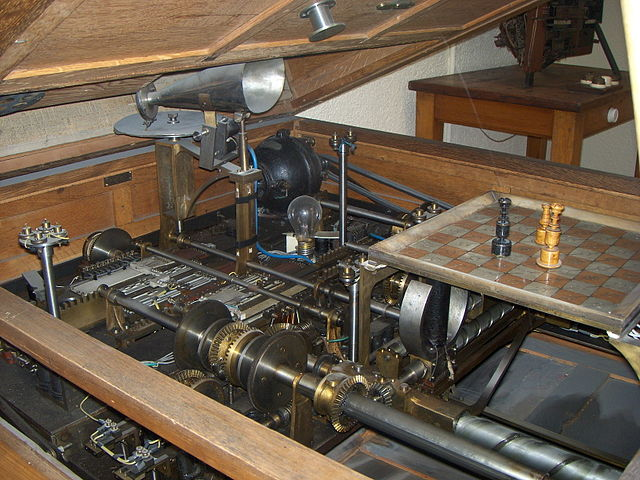
\includegraphics[width=0.7\linewidth]{ajedrecista.jpg}
        \captionof{figure}{El ajedrecista. Fuente: \href{https://es.wikipedia.org/wiki/El_Ajedrecista}{wikipedia}}
    \end{center}

    \item[1919]: Los inventores estadounidenses W. H. Eccles y F. W. Jordan desarrollan el primer circuito multivibrador o biestable (en léxico electrónico flip-flop). El flip-flop permitió diseñar Circuitos electrónicos que podían tener dos estados estables, alternativamente, pudiendo representar así el 0 como un estado y el otro con un 1. Esto formó la base del almacenamiento y proceso del \textbf{bit binario}, estructura que utilizan las actuales computadoras.

    \item[1924] Walther Bothe construye una puerta lógica \textbf{AND} para usarla en experimentos físicos, por lo cual recibió el premio Nobel de física en 1954.

    \item[1936] Alan Turing describe la máquina de Turing, la cual formaliza el concepto de algoritmo.

    \item[1938]: Konrad Zuse completa la primera computadora electromecánica, aunque no 100% operativa, la Z1.

    \item[1944] En Inglaterra se construyeron los ordenadores Colossus (Colossus Mark I y Colossus Mark 2), con el objetivo de descifrar las comunicaciones de los alemanes durante la Segunda guerra mundial.

    \item[1945] \href{https://es.wikipedia.org/wiki/John_von_Neumann}{John von Neumann} escribe el "First Draf of a report on the EDVAC" una página del primer documento donde se describe el diseño lógico de una computadora utilizando el concepto de programa almacenado (stored-program). Hoy día conocido como \textbf{Arquitectura de von Neumann}.

    \item[1946] En la Universidad de Pensilvania se construye la ENIAC (Electronic Numerical Integrator And Calculator), que fue la primera computadora electrónica de propósito general

    \begin{center}
        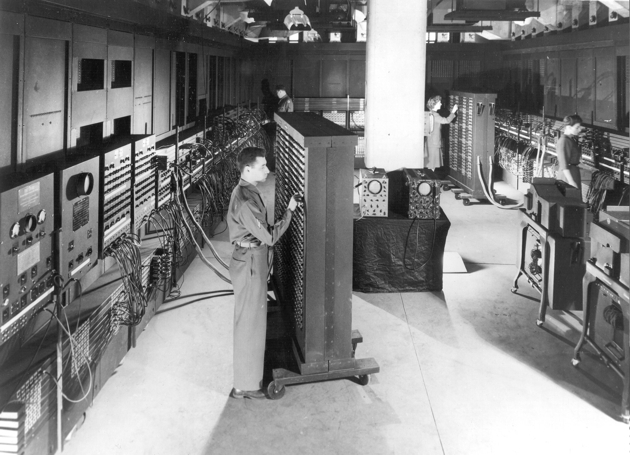
\includegraphics[width=0.7\linewidth]{ENIAC.jpg}
        \captionof{figure}{ENIAC. Fuente: \href{https://es.wikipedia.org/wiki/ENIAC}{wikipedia}}
    \end{center}

    \item[1951] El Sistema A-0 fue inventado por \href{https://es.wikipedia.org/wiki/Grace_Murray_Hopper}{Grace Murray Hopper}. Fue el \textbf{primer compilador} desarrollado para una computadora electrónica.

    \item[1958] Comienza la segunda generación de computadoras, caracterizados por usar \textbf{circuitos transistorizados} en vez de válvulas al vacío.

\end{description}

A partir de la década de los 60 se aceleran los avances, y cada año se crean nuevos sistemas que permiten evolucionar lo ya conocido.

\begin{description}
    \item[1964] La aparición del IBM 360 marca el comienzo de la tercera generación de computadoras. Comienzan las placas de circuitos integrados.

    \item[1969] Se publica el primer borrador de lo que será conocido como ARPANET (el precursor de la actual Internet).

    \item[1970] Intel crea la primera memoria dinámica RAM.

    \item[1971] Intel presenta el primer \textbf{procesador comercial} y a la vez el primer chip \textbf{microprocesador}, el Intel 4004.

    \item[1971] Ray Tomlinson crea el primer programa para enviar correo electrónico.

    \item[1974] Se crea el sistema Ethernet para enlazar a través de un cable único a las computadoras de una LAN.

    \item[1981] Se lanza al mercado el \textbf{IBM PC}, que se convertiría en un éxito comercial, marcaría una revolución en el campo de la computación personal y definiría nuevos estándares.

    \item[1981] Se termina de definir el protocolo \textbf{TCP/IP}. Lo utilizamos actualmente para navegar por Internet.

    \vspace{10pt}
    \begin{minipage}{0.75\linewidth}
        \item[1983] \href{https://es.wikipedia.org/wiki/Richard_Stallman}{Richard Stallman} anuncia públicamente el proyecto \href{https://es.wikipedia.org/wiki/GNU}{GNU}, con el objetivo de crear el primer sistema operativo libre de tipo Unix.
    \end{minipage}
    \hfill
    \begin{minipage}{0.15\linewidth}
        \hfill
        \includesvg[width=\linewidth]{gnu.svg}
    \end{minipage}

    \item[1986] El lenguaje \textbf{SQL} es estandarizado por ANSI.

    \item[1990] \href{https://es.wikipedia.org/wiki/Tim_Berners-Lee}{Tim Berners-Lee} idea el hipertexto para crear el World Wide Web (www) una nueva manera de interactuar con Internet.

    \begin{minipage}{0.8\linewidth}
        \item[1991] Linus Torvalds comienza a desarrollar Linux, el \textbf{kernel} (o núcleo) de un sistema operativo compatible con Unix.
    \end{minipage}
    \hfill
    \begin{minipage}{0.1\linewidth}
        \hfill
        \includesvg[width=\linewidth]{tux.svg}
    \end{minipage}

    \item[1991] Comienza a popularizarse la programación orientada a objetos.

    \item[1995] Aparece la primera versión de \href{https://es.wikipedia.org/wiki/MySQL}{MySQL}.

    \item[1995] Se inicia el desarrollo del servidor \href{https://es.wikipedia.org/wiki/Servidor_HTTP_Apache}{Apache}.

    \item[1997] EL IEEE crea la primera estándar WLAN y la llamaron 802.11. El primer protocolo para WiFi.

\end{description}

Se podrían añadir más momentos importantes hasta el día de hoy, pero como ya se ha dicho previamente, se ha elegido sólo un pequeño resumen.

\section{Componentes de un sistema informático}

Podemos diferenciar distintos componentes dentro de un sistema informático:

\begin{itemize}
    \item \textbf{Hardware}: Es todo lo que forma parte del ordenador, que \textbf{puede ser tocado físicamente}. Es decir: teclado, ratón, monitor, placa base, procesador, memoria, disco duro, cables, etc. Es la “maquinaria” necesaria utilizada para el tratamiento automático de la información.

    \item \textbf{Software}: Es el elemento lógico, es todo aquello que es “intangible”. Es el \textbf{conjunto de programas y datos} que permiten manejar el hardware, controlando y coordinando su funcionamiento para que realice las tareas deseadas.

    Dentro del software podemos diferenciar distintos tipos (aunque existen otras categorizaciones):

    \begin{itemize}
        \item \textbf{Software de sistema}: Son aquellos programas que permiten la administración del hardware (de los recursos físicos). Crean una capa de abstracción entre el hardware y los programas que utiliza el usuario. Dentro de este apartado podemos incluir: sistemas operativos, \textit{drivers} (controladores), herramientas de diagnóstico, ...

        \item \textbf{Software de desarrollo}: Son aquellos programas que los desarrolladores de software utilizan para crear, depurar y mantener programas.

        \item \textbf{Software de aplicación}: En esta categoría entran los programas que tienen una función específica y que normalmente son utilizados por los usuarios finales del sistema.
    \end{itemize}

\end{itemize}

A partir de aquí profundizaremos en cada uno de estos aspectos en los capítulos siguientes.